\documentclass{beamer}
\usepackage[utf8]{inputenc}

\usetheme{Madrid}
\usecolortheme{default}
\usepackage{amsmath,amssymb,amsfonts,amsthm}
\usepackage{txfonts}
\usepackage{tkz-euclide}
\usepackage{listings}
\usepackage{adjustbox}
\usepackage{array}
\usepackage{tabularx}
\usepackage{gvv}
\usepackage{lmodern}
\usepackage{circuitikz}
\usepackage{tikz}
\usepackage{graphicx}
 \graphicspath{{figs/}}
\setbeamertemplate{page number in head/foot}[totalframenumber]
\usepackage[T1]{fontenc}
\usepackage{lmodern}

\usepackage{tcolorbox}
\tcbuselibrary{minted,breakable,xparse,skins}



\definecolor{bg}{gray}{0.95}
\DeclareTCBListing{mintedbox}{O{}m!O{}}{%
  breakable=true,
  listing engine=minted,
  listing only,
  minted language=#2,
  minted style=default,
  minted options={%
    linenos,
    gobble=0,
    breaklines=true,
    breakafter=,,
    fontsize=\small,
    numbersep=8pt,
    #1},
  boxsep=0pt,
  left skip=0pt,
  right skip=0pt,
  left=25pt,
  right=0pt,
  top=3pt,
  bottom=3pt,
  arc=5pt,
  leftrule=0pt,
  rightrule=0pt,
  bottomrule=2pt,
  toprule=2pt,
  colback=bg,
  colframe=orange!70,
  enhanced,
  overlay={%
    \begin{tcbclipinterior}
    \fill[orange!20!white] (frame.south west) rectangle ([xshift=20pt]frame.north west);
    \end{tcbclipinterior}},
  #3,
}
\lstset{
    language=C,
    basicstyle=\ttfamily\small,
    keywordstyle=\color{blue},
    stringstyle=\color{orange},
    commentstyle=\color{green!60!black},
    numbers=left,
    numberstyle=\tiny\color{gray},
    breaklines=true,
    showstringspaces=false,
}
%------------------------------------------------------------
%This block of code defines the information to appear in the
%Title page
\title %optional
{1.4.23}
%\subtitle{A short story}

\author % (optional)
{Aniket-EE25BTECH11007}

\begin{document}


\frame{\titlepage}
\begin{frame}{Question}
Consider two points $P$ and $Q$ with position vectors 
\[
\vec{P} = 3\vec{a} - 2\vec{b}, \quad \vec{Q} = \vec{a} + \vec{b}.
\]
Find the position vector of a point $R$ which divides the line joining $P$ and $Q$ in the ratio $2:1$,
\begin{enumerate}
    \item internally, and 
    \item externally.
\end{enumerate}
\end{frame}

\begin{frame}{Theoretical Solution}
\noindent We write the endpoints in matrix form:
\begin{equation}
\myvec{\vec P \;\; \vec Q}^{T}
=
\myvec{3 \;\; -2 \\[2pt] 1 \;\; 1}
\myvec{\vec a \\[2pt] \vec b}.
\label{eq:endpoints}
\end{equation}

\noindent \textbf{General section formulas (matrix form).}
For points \(\vec A,\vec B\) and ratio \(k:1\):
\begin{equation}
\vec R_{\text{int}}
=\frac{k\,\vec B+\vec A}{k+1}
=\frac{1}{k+1}\,[\,\vec A\;\;\vec B\,]\,
\myvec{1\\ k}.
\label{eq:int_general}
\end{equation}
\begin{equation}
\vec R_{\text{ext}}
=\frac{k\,\vec B-\vec A}{k-1}
=\frac{1}{k-1}\,[\,\vec A\;\;\vec B\,]\,
\myvec{-1\\ k}.
\label{eq:ext_general}
\end{equation}
\end{frame}
\begin{frame}{Theoretical Solution}
\noindent \textbf{Internal division \(2:1\).}
Using \eqref{eq:int_general} with \(\vec A=\vec P,\ \vec B=\vec Q,\ k=2\),
\begin{equation}
\vec R_{\text{int}}
=\frac{1}{3}\,[\,\vec P\;\;\vec Q\,]\,
\myvec{1\\ 2}
=\myvec{\tfrac13 \;\; \tfrac23}\, \myvec{\vec P \;\; \vec Q}.
\label{eq:rint_def}
\end{equation}
Substitute \eqref{eq:endpoints} into \eqref{eq:rint_def}:
\begin{equation}
\vec R_{\text{int}}
=
\myvec{\tfrac13 \;\; \tfrac23}
\myvec{3 \;\; -2 \\[2pt] 1 \;\; 1}
\myvec{\vec a \\[2pt] \vec b}.
\label{eq:rint_sub}
\end{equation}
\begin{equation}
\boxed{\;\vec R_{\text{int}}=\tfrac{5}{3}\,\vec a\;}
\label{eq:rint_final}
\end{equation}
\end{frame}

\begin{frame}{Theoretical Solution}
    \noindent \textbf{External division \(2:1\).}
Using \eqref{eq:ext_general} with \(\vec A=\vec P,\ \vec B=\vec Q,\ k=2\),
\begin{equation}
\vec R_{\text{ext}}
=\,[\,\vec P\;\;\vec Q\,]\,
\myvec{-1\\ 2}
=\myvec{-1 \;\; 2}\,\myvec{\vec P \;\; \vec Q}.
\label{eq:rext_def}
\end{equation}
Substitute \eqref{eq:endpoints} into \eqref{eq:rext_def}:
\begin{equation}
\vec R_{\text{ext}}
=
\myvec{-1 \;\; 2}
\myvec{3 \;\; -2 \\[2pt] 1 \;\; 1}
\myvec{\vec a \\[2pt] \vec b}.
\label{eq:rext_sub}
\end{equation}
\begin{equation}
\boxed{\;\vec R_{\text{ext}}=-\,\vec a+4\,\vec b\;}
\label{eq:rext_final}
\end{equation}
\end{frame}

\begin{frame}[fragile]
    \frametitle{C Code - Internal and External Division}
    \begin{lstlisting}

#include <stdio.h>

// Function to find point dividing line in ratio m:n
// flag = 1 for internal, -1 for external
void sectionFormula(float Px, float Py, float Qx, float Qy, int m, int n, int flag,
                    float *Rx, float *Ry) {
    if(flag == 1) { // internal
        *Rx = (m*Qx + n*Px) / (float)(m+n);
        *Ry = (m*Qy + n*Py) / (float)(m+n);
    }
    else if(flag == -1) { // external
        *Rx = (m*Qx - n*Px) / (float)(m-n);
        *Ry = (m*Qy - n*Py) / (float)(m-n);
    }
}



    
     \end{lstlisting}
    \end{frame}


\begin{frame}[fragile]
    \frametitle{Python+C Code}
    \begin{lstlisting}
import ctypes
import matplotlib.pyplot as plt

# Load the shared library (make sure libsection.so is in the same folder)
lib = ctypes.CDLL("./mg1o.so")

# Define argument and return types
lib.sectionFormula.argtypes = [
    ctypes.c_float, ctypes.c_float,   # Px, Py
    ctypes.c_float, ctypes.c_float,   # Qx, Qy
    ctypes.c_int, ctypes.c_int,       # m, n
    ctypes.c_int,                     # flag (1=internal, -1=external)
    ctypes.POINTER(ctypes.c_float),   # Rx
    ctypes.POINTER(ctypes.c_float)    # Ry
]
lib.sectionFormula.restype = None
 \end{lstlisting}
\end{frame}
\begin{frame}[fragile]
    \frametitle{Python+C Code}
    \begin{lstlisting}
# Example points (P = (3,-2), Q = (1,1)), ratio 2:1
Px, Py = 3.0, -2.0
Qx, Qy = 1.0, 1.0
m, n = 2, 1

# Prepare storage for results
Rx_int, Ry_int = ctypes.c_float(), ctypes.c_float()
Rx_ext, Ry_ext = ctypes.c_float(), ctypes.c_float()

# Call C function
lib.sectionFormula(Px, Py, Qx, Qy, m, n, 1,  ctypes.byref(Rx_int), ctypes.byref(Ry_int))   # internal
lib.sectionFormula(Px, Py, Qx, Qy, m, n, -1, ctypes.byref(Rx_ext), ctypes.byref(Ry_ext))  # external

print("Internal Division:", Rx_int.value, Ry_int.value)
print("External Division:", Rx_ext.value, Ry_ext.value)
\end{lstlisting}
\end{frame}
\begin{frame}[fragile]
    \frametitle{Python+C Code}
    \begin{lstlisting}

# --- Plotting ---
plt.figure(figsize=(6,6))

# Plot P, Q, R_int, R_ext
plt.scatter([Px, Qx, Rx_int.value, Rx_ext.value],
            [Py, Qy, Ry_int.value, Ry_ext.value],
            color=["red","blue","green","purple"], s=100)

plt.text(Px+0.1, Py+0.1, "P", color="red")
plt.text(Qx+0.1, Qy+0.1, "Q", color="blue")
plt.text(Rx_int.value+0.1, Ry_int.value+0.1, "R_int", color="green")
plt.text(Rx_ext.value+0.1, Ry_ext.value+0.1, "R_ext", color="purple")
    \end{lstlisting}
\end{frame}
\begin{frame}[fragile]
    \frametitle{Python+C Code}
    \begin{lstlisting}
# Line PQ
plt.plot([Px, Qx], [Py, Qy], "k--")

plt.axhline(0, color="gray", linewidth=0.5)
plt.axvline(0, color="gray", linewidth=0.5)
plt.xlabel("Coefficient of a")
plt.ylabel("Coefficient of b")
plt.title("Section Formula using C + Python")
plt.grid(True)
plt.show()

    \end{lstlisting}
\end{frame}
\begin{frame}[fragile]
    \frametitle{Python}
    \begin{lstlisting}
import numpy as np
import matplotlib.pyplot as plt

# Point coordinates (coefficients of a and b)
Px, Py = 3.0, -2.0   # P = 3a - 2b
Qx, Qy = 1.0,  1.0   # Q = 1a + 1b
m, n = 2, 1          # ratio 2:1

# Internal Division: (mQ + nP) / (m+n)
Rx_int = (m*Qx + n*Px) / (m+n)
Ry_int = (m*Qy + n*Py) / (m+n)

# External Division: (mQ - nP) / (m-n)
Rx_ext = (m*Qx - n*Px) / (m-n)
Ry_ext = (m*Qy - n*Py) / (m-n)
\end{lstlisting}
\end{frame}
\begin{frame}[fragile]
    \frametitle{Python Code}
    \begin{lstlisting}
# Print results
print(f"Internal Division: R = {Rx_int:.2f}a + {Ry_int:.2f}b")
print(f"External Division: R = {Rx_ext:.2f}a + {Ry_ext:.2f}b")

# Plotting
plt.figure(figsize=(6,6))
plt.scatter([Px, Qx, Rx_int, Rx_ext],
            [Py, Qy, Ry_int, Ry_ext],
            color=["red","blue","green","purple"], s=100)

# Labels
plt.text(Px, Py, "P", fontsize=12, color="red")
plt.text(Qx, Qy, "Q", fontsize=12, color="blue")
plt.text(Rx_int, Ry_int, "R_int", fontsize=12, color="green")
plt.text(Rx_ext, Ry_ext, "R_ext", fontsize=12, color="purple")
\end{lstlisting}
\end{frame}
\begin{frame}[fragile]
    \frametitle{Python Code}
    \begin{lstlisting}
# Draw line PQ
plt.plot([Px, Qx], [Py, Qy], "k--", label="PQ")

# Axes styling
plt.axhline(0, color="gray", linewidth=0.5)
plt.axvline(0, color="gray", linewidth=0.5)
plt.xlabel("Coefficient of a")
plt.ylabel("Coefficient of b")
plt.legend()
plt.title("Section Formula Plot (Internal & External Division)")
plt.grid(True)
plt.show()
\end{lstlisting}
\end{frame}

\begin{frame}{Plot}
    \centering
    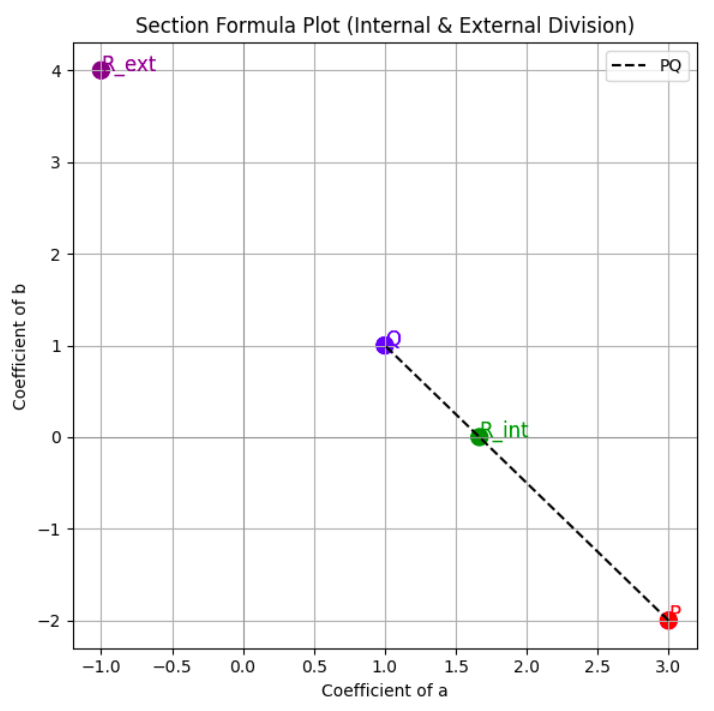
\includegraphics[width=\columnwidth, height=0.8\textheight, keepaspectratio]{figs/mg1plot.png}     
\end{frame}
\end{document}